% lec1.tex 
\chapter{General Theory of Ordinary Differential Equations}
\section{Generalities And Physical Motivation}
\lecture{1}{08:05 AM Sun, Sep 28 2025}{} 

An n$^{th} $-order ordinary differential equation (ODE for short) 
is a functional relationship having the form :
\[
F(t, x, x', \hdots , x^{(n)})  = 0
\]
The variable $t $ laying in the real interval $ I $ is commonly called the 
independent variable, and the $x \in C^{n}(I, \RR ^{k} )$ is the dependent 
variable. \\
An equation such as the above, is 
said to be in the implicit form. An ODE
is said to be in explicit form if 
it's written in the form: 
\[
x^{(n) } = 
f(t, x, x', \hdots , x^{(n-1) }) 
\]
Unfortunately, there is not too much to say about 
ODEs in the implicit form. Notice that such an equation 
can be reduced to the explicit form above, when the implicit function 
theorem applys.\\
\underline{\emph{Radioactive Desintegration:}} \\ The law of radiocative desintegration
have been formulated in \textbf{1902} by constating that the instantaneous 
rate of desintegration of a given radiocative element is propotional to the
number of atoms existings at the time considered, and doesnt 
depend on any other external factors. we write: 
\[
  X'(t)  = - a x(t)  \quad \quad \quad \quad \quad \quad 
  ( x(t) = x(0) e^{-at}   ) 
\]
where $x(t)$ is the number of non desintegrated atoms at time $t$, 
the positive constant is called desintegration constant and is related to the 
radiocative element and is experminetally determined.\\
\underline{\emph{Mathematical Pendulum:}} \\ Consider a pendulum of length $l $ and denote by $\DD  (t)  $ the length of the 
arc described by the free extrimity at time $t$. we have $s(t) = l x(t)   $ is
the measure in the radian of the angle between the vertical axis and the pendulum. \\
$\vec{P} = mg  $  is the force exercised upon the pendulum. Decomposing the force $\vec{P}  $ 
on the tangential axis and the thread axis and considering that the component of $\vec{P}  $ is
conunter-balanced by the resistance of the resistance of the thread, we obtain by
Newtons second law:
\[
m l x'' = -mg \sin{(x) }
\]
thus we get: 
\[
x'' + \frac{g}{l} \sin{ (x) } = 0
\]
\underline{\emph{A Spatial Model in Ecology:}} 
\[
x' = \lm x (1 - x)  - x
\]
we have an infinite number of sites linked by immigration, all the sites are equally accessible
$x(t)$ is the number of occupied sites and assume that the time is scalled 
so that the rate at which the sites become vaccout equals $1$. \\
$x^{'} $ is propotional to the product of the occupied sites and vaccout sites. \\
\underline{\emph{The Prey Predator Model (Dynamic of population):}} 
\[
\begin{cases}
x' = (a - hy) x \\
y' = -(b - kx) y 
\end{cases}
\quad \quad 
\quad 
\text{Lotha Volterra System} 
\]
\begin{itemize}
  \item $x $ is the population of prey species 
    \item $y $ is the population of predator species 
\end{itemize}
\underline{\emph{R.L.C Circuit:}} 
\\
\\
\\
$\quad \quad \quad  $ 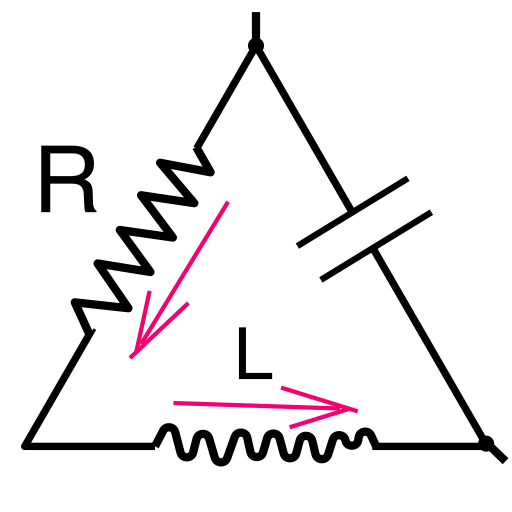
\includegraphics[width=0.2\textwidth]{images/rl1.png}
\[
  \begin{cases}
  \mathcal{L}  \quad 
  i_{L}' (t) = v_{L} - g(i_{L})   \\
  \mathcal{C} \quad 
  v_{c}'(t) = - i_{L} 
  \end{cases}
\]
$\vec{i}(t) = (i_{k}(t), i_{L}(t), i_{C}(t)  )$ is the state of the current 
in the circuit.\\
$v(t) = (v_{k}(t) , v_{L}(t) , v_{C}(t) )  $ is the state of the volatage in the circuit, 
the above is obtained by, Kirochoff, Faraday and Ohm Laws.
\section{Initial Value Problem (or Cauchy Problem)}
We start by following remark. Any explicit ODE of n$^{th} $-order $(n \geq 2)$ can be reduced 
to a first order ODE in explicit form. Indeed, 
\[
  x^{(n) }  = f(t, x, x', \hdots , x^{(n-1) }) 
\]
Put $U = (u_1, u_2, \hdots , u_{n})  $, where: 
\[
\begin{cases}
u_1 = x \\
u_2 = x' \\
\quad  \vdots \\
u_{n} = x^{(n-1) }
\end{cases}
\]
Notice:
\[
U' = (u_1', u_2', \hdots , u_{n}')  = 
(x', x'', \hdots , x^{(n) }) 
\]
Thus:
\[
U' = (u_2, u_3, \hdots , u_{n-1}, f(t, U) )  = \overline{f}(t, u) 
\]
Hence, from now on, we consider only $1^{st}$-order ODEs. \\
In all what follows, we let $\Omega \subset \RR  \times \RR ^{k}$ is a domain, and 
$ f : \Omega  \longrightarrow \RR ^{k} $ a continuous function.
\begin{definition}[]
An initial value problem (IVP for short) or a Cauchy is given by: 
\[
\begin{cases}
x' = f(t, x)  \\
x(t_0) = x_0 
\end{cases}
\]
where $(t_0, x_0) \in \Omega $ 
\end{definition}
\begin{definition}[]
A function $ \FF  : I \longrightarrow \RR ^{k} $ of class $\mathcal{C} ^{1} $ on the real
interval $I $ is a solution of the IVP (I.1) if 
$(t, \FF (t) )  \in  \Omega $, and $\FF '(t) = f(t, \FF (t) )   $ for all
$t \in  I $. 
\end{definition}
\begin{definition}[]
  Let $ \FF  : I \longrightarrow \RR ^{k} $ be a solution of the IVP (I.1). The form: 
  \[
    \FF (t) =  x_0 + \int_{t_0}^{t} f(s, \FF (s) )  ds
  \]
  is called the integral form of the solution.
\end{definition}
% end of ui1e
